\begin{enumerate}
    \item Vysvětlete, jak nalézt pozice volných bodů
    \[\lr{x_1, y_1}, \lr{x_2, y_2}, \dots, \lr{x_n, y_n} \]
    tak, aby minimializovaly kvadrát součtu jejich délek.

    \noindent\rule{\textwidth}{1pt}

    Máme zadanou sumu kvadrátů délek:
    \[ \sum_{k = 1}^K \left[ \lr{x_{I \lr{k}} - x_{J \lr{k}}}^2 + \lr{y_{I \lr{k}} - y_{J \lr{k}}}^2 \right], \]
    kde \(I \lr{k}\), resp. \(J \lr{k}\ \), označuje index počátečního, resp. koncovýho, uzelu hrany.

    Ze zadané sumy je vidět, že jednotlivé souřadnice jsou na sobě nezávislé a tedy je lze optimalizovat každou zvlášť.

    Na začátku máme zadanou matici \bf{A}, která v řádcích obsahuje index bodu, ve kterém hrana začíná, a index bodu, ve kterém hrana končí. Počáteční, resp. koncový, uzel je v matici označen jako \( 1 \), resp. \( -1 \).
    Matice obsahuje \( k \) řádků, kde číslo \( k \) označuje počet hran mezi body.
    
    Ze zadání je známo, kolik bodů je fixních a kolik volných. Díky tomu lze z matici rozdělit na dvě části, kde v jedné části budou body volné a v druhé body fixní
    \[ \bf{A} = \left[ \bf{A}_? \, \bf{A}_F \right]. \]

    Po této úpravě dostáváme následující výraz
    \[
        \left[ \bf{A}_? \, \bf{A}_F \right] \cdot
        \begin{bmatrix}
            x_1 \\
            \vdots \\
            x_n \\
            -- \\
            x_{n + 1}\\
            \vdots \\
            x_N
        \end{bmatrix}      
    \]

    Z něj je vidět, že matice \( \bf{A}_? \) má rozměry \( k \times n \) a matice \( \bf{A}_F \) má rozměry \( k \times \ N - n \), kde \( N \) je celkový počet bodů (uzlů).

    Pokud tento výraz upravíme a položíme rovný 0, získáme rovnici, která lze převést na optimalizační úlohu minimalizace

    \[
        \left[ \bf{A}_? \, \bf{A}_F \right] \cdot
        \begin{bmatrix}
            x_1 \\
            \vdots \\
            x_n \\
            -- \\
            x_{n + 1}\\
            \vdots \\
            x_N
        \end{bmatrix}
        =
        \left[ \bf{A}_? \, \bf{A}_F \right] \cdot
        \begin{bmatrix}
            x_{?} \\
            x_{F}
        \end{bmatrix}
        = \bf{A}_? \cdot x_? + \bf{A}_F \cdot x_{F}
    \]

    \begin{align*}
        \bf{A}_? \cdot x_? + \bf{A}_F \cdot x_{F} &= 0 \\
        \bf{A}_? \cdot x_? &= \lr{-1} \cdot \bf{A}_F \cdot x_{F}
    \end{align*}
    z čehož dostáváme optimalizační úlohu
    \[    
        \min \lVert \bf{A}_? - \bf{A}'_F \cdot x_{F} \rVert,
    \]
    kde \( \bf{A}'_F = \lr{-1} \cdot \bf{A}_F \).

    \noindent\rule{\textwidth}{1pt}

    \item Napište program pro Matlab, který daný úkol vyřeší pro zadané hodnoty.

    Zadané hodnoty nejsou zobrazeny, pouze doplněný kód.

    \begin{lstlisting}
% Afree = A_?, Afixed = A_F
Afree = A(:,1:n);
Afixed = A(:,(n+1):end);

xfree = Afree \ (Afixed * xfixed * -1);
yfree = Afree \ (Afixed * yfixed * -1);
    \end{lstlisting}

    Výsledek je \verb|ans = 22.2237|.
\end{enumerate}

\begin{center}
    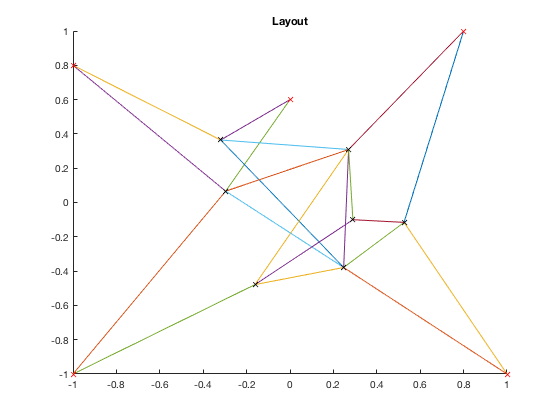
\includegraphics[width=0.75\textwidth]{quadratic_placement.png}
\end{center}

